\clearpage
\section*{Decode}
\noindent
The Decode block provides access to the register file, as well as interpreting instructions from Fetch to regulate read and access. The Decode block accepts \verb+iCode+, \verb+rA+, \verb+rB+, \verb+valM+, \verb+valE+, \verb+dstM+, and \verb+dstE+ as input (as well as a clock signal). It returns \verb+valA+ and \verb+valB+.\\\\
Decode is comprised of three primary subsections: the register file, \verb+srcA+, and \verb+srcB+.\\\\
The register file provides output to \verb+valA+ and \verb+valB+ based on the registers it is instructed to read. Using \verb+iCode+, \verb+srcA+ and \verb+srcB+ determine if a register needs to be read, and passes along the address from \verb+rA+ or \verb+rB+ respectively if so.\\\\
The register file can also be modified using \verb+dstM+, \verb+dstE+, \verb+valM+, and \verb+valE+. If the \verb+WriteEnable+ is enabled, the register file will update the corresponding destination with its appropriate value. The \verb+MEDecoder+ helps determine which of E or M should be written to, since only one can happen at a time. 

\subsection*{Contributors}
Kyle Crusius

\subsection*{Screenshots}

\begin{figure}[!ht]
    \centering
    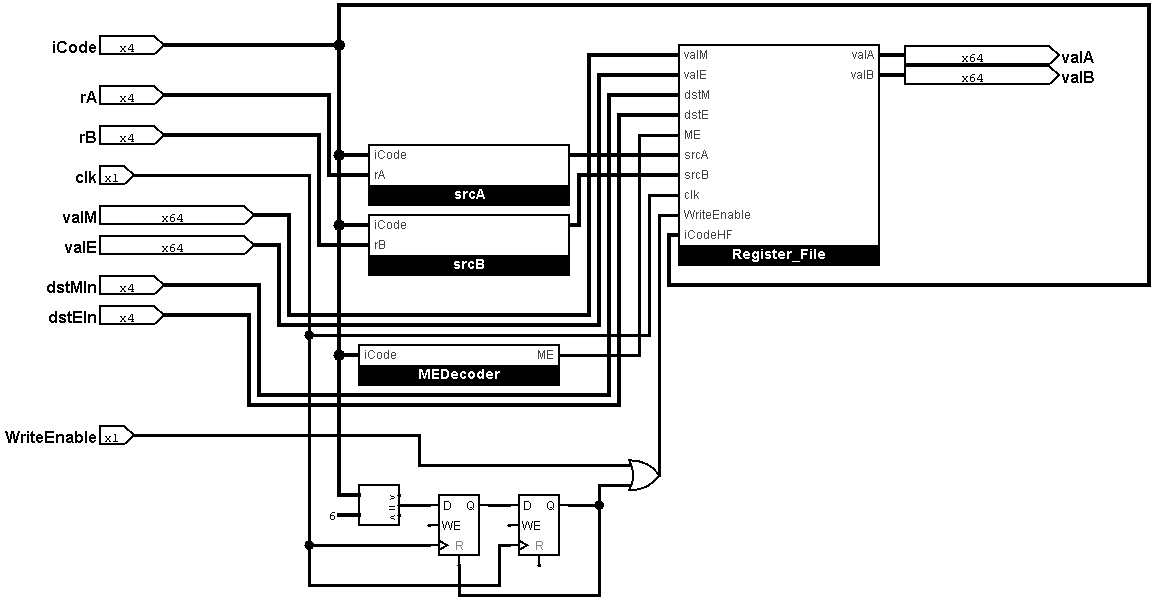
\includegraphics[width=\textwidth]{Images/Decode.png}
    \caption{Decode}
\end{figure}